% PDF 101
\sourcepage{97}{101}
它将在第二部分结构层的构造中起重要作用。

这个典范基对有限交封闭。确切地说，
\begin{equation}\tag{3.7}
X_{fg}=X_f\cap X_g\qquad\forall(f,g)\in A\times A.
\end{equation}
基开集之间的包含关系可以用交换代数来解释。例如：$X_f\subset X_g$ 蕴涵存在正整数 $n$ 和元素 $h\in A$，使
\begin{equation}\tag{3.8}
g^n=hf.
\end{equation}
\footnote{译注：原文此式的 $f,g$ 次序颠倒。按 $X_f=\Spec A\setminus V(f)$ 的定义，正确条件为 $f^n=hg$。以下涉及包含关系时均须注意这一点。}
\textit{证明。}原文给出的推导为
\[
X_f\subset X_g\iff V(f)\supset V(g)
\iff V(fA)=V(\sqrt{fA})\supset V(g)\Longrightarrow(3.8).
\]
特别地，$A$ 中两个元素 $f,g$ 定义同一个基开集 $X_f=X_g$，当且仅当存在整数 $m>0,n>0$，使 $f^m\in Ag$、$g^n\in Af$。

［我们之所以强调典范基 $\mathcal B=\{X_f\}_{f\in A}$，是因为把 $X$ 上的层刻画为特殊预层的正合性条件，可以用交换代数来表述。为把这一点说清楚，我在这里依据录音记下格罗滕迪克的讲述，以免在构造结构层 $\widetilde A$ 时插入过多冗长的题外讨论（参见本章第二部分第6、7、8节等）。］

……在讨论 $\Spec A$ 上的环结构层 $\widetilde A$ 之前（参见第三章第二部分），我先利用前面提到的性质，对谱上的层作一般描述：形如 $X_f\in\Ob\mathcal B$（$f\in A$）的开集构成一个对有限交封闭的拓扑基。再次回顾，在任意拓扑空间 $X$ 上给出一个集合层，等价于给出一个满足某些正合性条件的预层。首先，对任何拓扑空间 $X$，都可以构造范畴 $\operatorname{Op}(X)$（见原书第95页脚注），它的对象是 $X$ 的开集。对于两个开集 $U,V$，若 $U\not\subset V$，则态射集 $\Hom(U,V)$ 为空；若 $U\subset V$，则它只含唯一的态射 $i_V^U:U\to V$，即典范包含映射。

% PDF 102
\sourcepage{98}{102}
$X$ 上取值于范畴 $C$ 的预层 $P$，是一个反变函子
\[
P:\operatorname{Op}(X)^{\op}\longrightarrow C.
\]
格罗滕迪克此时特别关心 $C$ 为集合范畴的情形。

……$X$ 上的集合层 $F$ 是这样一种预层：它给 $X$ 的每个开集 $U$ 配以一个集合 $F(U)$；而且，只要 $U$ 被开集 $U_i$（$i\in I$）覆盖，
\begin{equation}\tag{3.9}
U=\bigcup_{i\in I}U_i,
\end{equation}
考虑各交集 $U_i\cap U_j$（$i,j\in I$），由限制映射 $\rho_{U_i}^U:F(U)\to F(U_i)$ 的乘积，以及对应于 $U_i\cap U_j$ 到 $U_i$、$U_j$ 的两个包含映射，便得到正合序列
\begin{equation}\tag{3.10}
F(U)\longrightarrow\prod_{i\in I}F(U_i)
\rightrightarrows\prod_{i,j\in I}F(U_i\cap U_j).
\end{equation}
\footnote{这里的正合性是指，单箭头的像等于双箭头的核。在集合范畴中，双箭头 $A\mathrel{\substack{\xrightarrow{u}\\[-.6ex]\xrightarrow{v}}}B$ 的核定义为 $\ker(u,v)=\{a\in A\mid u(a)=v(a)\}$。在一般范畴中，用对象的态射代替对象的点，就把定义归结为集合情形。}
换言之，预层 $F$ 为层，等价于对于每个开集 $U$ 及其每个开覆盖 (3.9)，序列 (3.10) 都正合。

现在回到 $X=\Spec A$。由于 $\mathcal B$ 是对有限交封闭的基（见 (3.7)），只须用对应 $X_f\mapsto F(X_f)$（$f\in A$，$X_f\in\mathcal B$）改写上述一般讨论。只要 $X_f$ 被开集 $X_{f_i}$（$f_i\in A$）覆盖，
\begin{equation}\tag{3.11}
X_f=\bigcup_{i\in I}X_{f_i}\qquad(f,f_i\in A,\ i\in I),
\end{equation}

% PDF 103
\sourcepage{99}{103}
考虑交集 $X_{f_i}\cap X_{f_j}$（$i,j\in I$），将 $F(X_f)$ 映入各限制的乘积，再由两个包含映射 $X_{f_i}\cap X_{f_j}\subset X_{f_i},X_{f_j}$ 映入相应乘积，便得到图式
\begin{equation}\tag{3.12}
F(X_f)\longrightarrow\prod_{i\in I}F(X_{f_i})
\rightrightarrows\prod_{i,j\in I}F(X_{f_if_j}),
\end{equation}
其正合性的含义是显然的。

为用交换代数表述，我们简化记号，把待描述的“层”记为 $G$，并置
\begin{equation}\tag{3.13}
G(f)=F(X_f)\qquad\forall f\in A.
\end{equation}
这样，环 $A$ 的每个元素 $f$ 都对应一个集合 $G(f)$。\footnote{依 $G$ 所取值的范畴而定，$G(f)$ 也可以是群、环、$A$-模等。正文中的 $F(f)$ 暂且仍只是集合。}我们要给这族集合 $\{G(f)\}_{f\in A}$ 配备一些数据，并规定这些数据应满足的条件，使之定义一个“层” $G$。

具体条件如下：
\begin{enumerate}[label=\alph*)]
\item 对每个 $f\in A$，给出 $f\mapsto G(f)$。
\item 对满足 $X_f\subset X_g$ 的每一对元素 $f,g\in A$，给出限制映射
\[
\rho_f^g:G(g)\longrightarrow G(f).
\]
\end{enumerate}
我们必须用交换代数解释 $X_f\subset X_g$ 的含义。前面已经看到（原书第97页），这等价于存在正整数 $n$ 和 $h\in A$，满足 (3.8) 所表达的整除条件。也就是说，$X_f\subset X_g$ 可以用环 $A$ 中的整除关系表述。此外，还须满足传递性：若 $X_f\subset X_g\subset X_h$，相应的限制映射图式

% PDF 104
\sourcepage{100}{104}
\begin{equation}\tag{3.14}
\begin{tikzcd}[ampersand replacement=\&]
G(h)\arrow[r]\arrow[dr] \&G(g)\arrow[d]\\
\&G(f)
\end{tikzcd}
\end{equation}
交换。于是我们得到“基开集 $X_f$ 所成范畴上的预层”，它又可以解释为 $A$ 这个范畴上的预层［参见下文关于“景”的插叙］；这里的范畴结构来自整除这一预序关系。\footnote{［把这一口头讲述形式化如下：$F:\operatorname{Op}(X)^{\op}\to\Sets$ 定义在 $X$ 的开集范畴上；$G$ 则由环 $A$ 的元素给出。然而，说 $G:A^{\op}\to\Sets$ 是反变函子是有意义的，因为关系 $g\mid f\iff\exists n\geq0,h\in A,\ f^n=hg$ 在 $A$ 上定义了范畴结构：若此关系不成立，则 $\Hom_A(g,f)=\varnothing$；若成立，则有唯一的态射。这是一个预序关系。］这里的“整除”采用原文所述的幂整除意义。}

预层本身尚没有多少拓扑意义，因此还要引入正合性，把相应条件用交换代数写出。确切地说：对每个 $f\in A$ 和每族元素 $f_i\in A$（$i\in I$），若 $X_f=\bigcup_{i\in I}X_{f_i}$，就要求由限制态射构成的图式
\begin{equation}\tag{3.15}
G(f)\longrightarrow\prod_{i\in I}G(f_i)
\rightrightarrows\prod_{i,j\in I}G(f_if_j)
\end{equation}
正合。这个条件要对每个 $f$、每个开覆盖成立；也就是说，$G(f)$ 应当能够与乘积 $\prod_{i\in I}G(f_i)$ 中被两个箭头映为同一元素的那些元素所成的子集等同起来。

现在用交换代数解释这些条件：
\begin{enumerate}[label=\alph*)]
\item 对每个 $X_{f_i}\subset X_f$，回顾这意味着存在 $n_i\geq0$、$h_i\in A$，使 $f_i^{n_i}=fh_i$。也就是
\[
\bigcup_{i\in I}X_{f_i}\subset X_f
\iff
\forall i\in I,\quad f_i^{n_i}=fh_i
\quad\text{（某些 $n_i,h_i$）}.
\]
\end{enumerate}

% PDF 105
\sourcepage{101}{105}
\begin{enumerate}[label=\alph*),start=2]
\item 还须表达反向的包含关系 $X_f\subset\bigcup_{i\in I}X_{f_i}$。这意味着 $V(f)\supset\bigcap_{i\in I}V(f_i)$，亦即 $V(fA)\supset\bigcap_iV(f_iA)$，从而涉及根理想 $\sqrt{fA}$ 和 $\sqrt{\sum_i f_iA}$ 之间的包含关系：
\begin{equation}\tag{3.16}
V(\sqrt{fA})\supset V\left(\sqrt{\sum_{i\in I}f_iA}\right).
\end{equation}
这等价于存在整数 $n\geq0$ 及有限多个元素 $g_i\in A$，使
\begin{equation}\tag{3.17}
f^n=\sum_i g_if_i.
\end{equation}
\end{enumerate}
至此，一切都已用交换代数解释了！实际上，我们已经用交换代数重新构造了形如 $X_f$ 的开集所成的“景”。\footnote{我们的这位朋友忘了，并不是每个人都听过他的拓扑斯课程（理解本课程也并不需要那门课）；不过他补了一句简短的解释：“景不过是一个范畴加上覆盖数据。”景也就是“格罗滕迪克拓扑”：在一个存在纤维积的范畴中，只要把 $X$ 内的交集 $U_i\cap U_j$ 换成 $U_i\times_XU_j$，就能表述覆盖的基本性质。纤维积的正式定义见第二章第1、2节。关于格罗滕迪克拓扑，最简明的介绍可见 Dieudonn\'e，\textit{Advances II}，第407--411页。}

典范基还有一个后面要用的重要性质，即函子性。第4节将证明它。

\Section{4}{函子 $\Spec$}
前面第1、2、3节中，我们固定了 $X=\Spec A$。现在来验证，在含幺交换环的范畴 $\G$ 中，每个态射
\begin{equation}\tag{4.1}
u:A\longrightarrow B
\end{equation}
都对应谱之间一个方向相反的连续映射
\begin{equation}\tag{4.2}
\Spec u:\Spec B\longrightarrow\Spec A.
\end{equation}
我们已经知道如何定义底集之间的映射
% PDF 106
\sourcepage{102}{106}
$\mathfrak b\mapsto u^{-1}(\mathfrak b)$。只须验证 $\Spec u$ 连续。设 $V(S)$ 是 $\Spec A$ 的闭集（$S\subset A$）。条件
\[
(\Spec u)(\mathfrak b)=u^{-1}(\mathfrak b)\in V(S)
\]
等价于 $u^{-1}(\mathfrak b)\supset S$，亦即 $\mathfrak b\supset u(S)$，也就等价于 $\mathfrak b\in V(u(S))$。因此，$\Spec A$ 中闭集 $V(S)$ 在 $\Spec u$ 下的逆像是 $V(u(S))$，它在 $\Spec B$ 中是闭的。

\textbf{诱导映射 $\Spec u$ 是连续映射。$\Spec$ 是从含幺交换环及保幺环同态组成的范畴 $\G$ 到拓扑空间及连续映射范畴的反变函子。}

作为 (4.1) 的特例，考虑典范满同态 $u:A\to A/\mathfrak a$，$a\mapsto a+\mathfrak a$，其中 $\mathfrak a$ 为 $A$ 的理想。那么 $\Spec u:\Spec(A/\mathfrak a)\to\Spec A$ 是谱之间的典范单射。

若 $\mathfrak a=\operatorname{Nil}A$ 是 $A$ 的幂零根，则由 $\mathfrak p\mapsto\mathfrak p/\operatorname{Nil}A$ 定义的底集之间的双射，实际上是两个拓扑空间之间的同胚：
\begin{equation}\tag{4.3}
\Spec A\simeq\Spec(A/\operatorname{Nil}A).
\end{equation}
仅此性质就足以说明，不能从 $\Spec A$ 恢复 $A$。$A$ 是域的情形更为鲜明：任意域 $k$ 的谱都是单点空间，这一点对应 $k$ 的唯一素理想 $(0)$，即 $\Spec k=\{(0)\}$。

现在证明，由 (4.1) 诱导的连续映射 (4.2) 把 $Y$ 的基开集（见第3节）通过逆像送到 $X$ 的基开集。事实上，开集 $Y_f$（$f\in A$）的逆像 $\varphi^{-1}(Y_f)$ 在 $X$ 中开。我们将证明下述函子性：

% PDF 107
\sourcepage{103}{107}
\begin{equation}\tag{4.4}
\varphi^{-1}(\mathcal B_Y)=\mathcal B_X
\qquad\text{（$\mathcal B_X,\mathcal B_Y$ 分别为 $\operatorname{Op}(X),\operatorname{Op}(Y)$ 的典范基）},
\end{equation}
\footnote{译注：一般只能断言 $\varphi^{-1}(\mathcal B_Y)\subset\mathcal B_X$；原文 (4.4) 的等号过强。下式 (4.5) 是所需的精确结论。}
而且有更漂亮、更精确的形式：对每个 $f\in A$、$Y_f\in\mathcal B_Y$，
\begin{equation}\tag{4.5}
\varphi^{-1}(Y_f)=X_{u(f)}.
\end{equation}
回到格罗滕迪克在课堂上使用的第3节的简化记号，暂不采用本节的函子式记号：重新置 $X=\Spec B$、$Y=\Spec A$、$\varphi=\Spec u$，这样，$\Spec$ 将 $A\xrightarrow{u}B$ 变为 $Y\leftarrow X$。任取对应于元素 $f\in A$ 的基开集 $Y_f\in\mathcal B_Y$，则
\begin{equation}\tag{4.6}
\begin{aligned}
Y_f&=\{\mathfrak p\in\Spec A\mid f\notin\mathfrak p\},\\
\varphi^{-1}(Y_f)
&=\{\mathfrak q\in\Spec B\mid\varphi(\mathfrak q)\in Y_f\}\\
&=\{\mathfrak q\in\Spec B\mid u^{-1}(\mathfrak q)\in Y_f\}\\
&=\{\mathfrak q\in\Spec B\mid f\notin u^{-1}(\mathfrak q)\}\\
&=\{\mathfrak q\in\Spec B\mid u(f)\notin\mathfrak q\}=X_{u(f)}.
\end{aligned}
\end{equation}
证毕。换言之，$Y$ 的典范基 $\mathcal B_Y$ 在 $\varphi^{-1}$ 下自然映入 $X$ 的典范基 $\mathcal B_X$，并满足 (4.5)。

为了恢复 $A$，我们将在第二部分定义 $\Spec A$ 上的结构层 $\widetilde A$，使
\[\Gamma(\Spec A,\widetilde A)\simeq A.\]
届时将看到，这些取值于环范畴的层起着根本作用。

\Section{5}{适用于 $\Spec A$ 的点集拓扑插叙及例子}
古典代数几何中的若干重要概念，实际上是适用于任意拓扑空间的纯拓扑概念。这里借助扎里斯基拓扑，把它们用于代数几何中远非豪斯多夫的空间：代数簇、概形等等。点集拓扑课程通常不讨论这些概念，因为在被视为“自然”空间的豪斯多夫空间中，它们变得平凡。这里所需的 $T_0$、$T_1$ 空间往往被当作“病态”而受到忽视。然而，代数几何的研究对象自然且重要，这些空间又在其中起如此重大的作用，我们很有必要克服这种成见。格罗滕迪克下面讨论的典型概念有：不可约性、一般点（前面已提及）、特化、清醒空间等。更多细节见 EGA，Springer 版，第0章第2节，第48页。

\textbf{格罗滕迪克的概要。}现在我要证明，谱 $X=\Spec A$ 是一个清醒空间，

% PDF 108
\sourcepage{104}{108}
也就是说，对 $X$ 的每个不可约闭子空间 $Y$，都存在一点 $y\in Y$，使 $Y=\overline{\{y\}}$。\footnote{参见 (5.1) 给出的不可约性的拓扑定义。这个定义与老一辈使用的相同；“新”意在于把旧定义看成一般拓扑概念，并应用到扎里斯基拓扑上。}按照前面的定义和说明，每个不可约闭子空间都有且仅有一个一般点。换言之，$x\mapsto\overline{\{x\}}$ 给出了 $X$ 的点集与 $X$ 的不可约闭子空间族之间的一一对应。

称拓扑空间 $X$ \textbf{不可约}，如果 $X$ 非空，而且不能写成两个都不同于 $X$ 的闭集的并：
\begin{equation}\tag{5.1}
\begin{gathered}
X\ne\varnothing,\qquad X=X'\cup X'',\qquad
X'=\overline{X'},\quad X''=\overline{X''}\\
\Longrightarrow\quad X'=X\ \text{或}\ X''=X.
\end{gathered}
\end{equation}
［\textbf{注。}不可约性与连通性并不完全相同，因为这里没有假定 $X'\cap X''=\varnothing$。换言之，不可约空间总是连通的，反之却不成立。例如仿射平面中两条不同且相交的直线 $A,B$ 的并 $A\cup B$，它连通，却不是不可约的。］

子空间 $Y\subset X$ 不可约，当且仅当对于 $X$ 中的闭集 $A,B$，$Y\subset A\cup B$ 蕴涵 $Y\subset A$ 或 $Y\subset B$。因此，$Y\subset X$ 不可约，当且仅当其闭包 $\overline Y$ 不可约；也就是说，不可约性在取闭包下保持。

对任何 $X$，单点集 $\{x\}\subset X$ 都不可约。前面已经看到，在 $\Spec A$ 中，$\{x\}$ 不一定闭；亦即 $\Spec A$ 不一定是 $T_1$ 空间。因而，我们必须容许 $\overline{\{x\}}$ 比 $\{x\}$ 更大（而且常常“大得多”，见本节末的例子）。由刚才的说明，单点集的闭包 $\overline{\{x\}}$ 总是不可约的。反过来，设 $V$ 是 $X$ 的不可约子空间，若 $x\in V$ 满足 $V=\overline{\{x\}}$，就称 $x$ 是 $V$ 的\textbf{一般点}（$\Spec A$ 的特例见第3节）。

若 $y\in\overline{\{x\}}$，则每个含 $x$ 的闭集 $F$ 也含 $y$；等价地，

% PDF 109
\sourcepage{105}{109}
$y$ 的每个开邻域都含 $x$。若 $X$ 是 $T_0$ 空间（柯尔莫哥洛夫空间），它的每个不可约子空间至多含一个一般点。这是因为，若 $\overline{\{x\}}=\overline{\{y\}}=V$ 且 $x\ne y$，则 $x$ 的每个开邻域都含 $y$，而 $y$ 的每个开邻域都含 $x$，这与 $T_0$ 性质矛盾（见原书第90页脚注）。若 $y\in\overline{\{x\}}$，就说 $y$ 是 $x$ 的\textbf{特化}，亦即 $x$ 是 $y$ 的\textbf{一般化}。

若拓扑空间 $X$ 的每个不可约子空间 $Y$ 都有一般点，就称 $X$ \textbf{清醒}。\footnote{译注：这里及随后的一一对应中的“不可约子空间／子集”均应限于不可约\emph{闭}子空间；原文这几处省略了“闭”，本节开头已明确写出。另依现代通常约定，清醒性本身即包括一般点的唯一性。}若 $X$ 既为 $T_0$ 又清醒，则 $X$ 的每个不可约子空间都有且仅有一个一般点。换言之，在 $T_0$ 的清醒空间 $X$ 中，$x\mapsto\overline{\{x\}}$ 是 $X$ 的点与不可约子集之间的双射。

若 $f:X\to Y$ 连续，源空间 $X$ 不可约，则目标空间中的像 $f(X)$ 也不可约。

对于豪斯多夫空间，不可约性并没有多少内容：豪斯多夫空间 $X$ 不可约，当且仅当 $X$ 恰含一个点！

［事实上，定义性质 (5.1) 的集合论对偶是：$X$ 中任意两个非空开集相交（见第一章第14节），即
\[
A,B\text{ 开},\quad A\ne\varnothing,\ B\ne\varnothing
\quad\Longrightarrow\quad A\cap B\ne\varnothing.
\]
\footnote{也可将这一性质作为不可约性的定义。其他等价条件为：1）$X$ 的每个非空开集 $A$ 在 $X$ 中稠密，即 $\overline A=X$；2）$X$ 的每个开子空间都连通。简单的验证留给读者。}
所以，一个含有两个不同点的不可约空间不可能是豪斯多夫的：若 $P,Q$ 是豪斯多夫空间中两个不同的点，它们就有不相交的开邻域，从而 $X$ 不可能不可约。］

代数几何中的情形当然截然不同！例如，对古典仿射代数簇 $X$，$X$ 不可约，当且仅当 $X$ 上的多项式函数环是整环。

这些概念可以立即用于赋予谱拓扑的 $\Spec A$（$A\in\Ob\G$，见第2节）。若 $X$ 是环 $A\in\Ob\G$ 的谱，我们要弄清楚

% PDF 110
\sourcepage{106}{110}
$X$ 不可约意味着什么。首先注意，把 $A$ 换成 $A/\operatorname{Nil}A$ 不改变谱，因为每个素理想都含 $\operatorname{Nil}A$，而 $\mathfrak p\mapsto\mathfrak p/\operatorname{Nil}A$（$\mathfrak p\in\Spec A$）给出 $\Spec A$ 与 $\Spec(A/\operatorname{Nil}A)$ 之间保持拓扑的双射。

因此，为了判断不可约性，可以假定 $A$ 是约化环。分别验证不可约性的两个条件：$X=\Spec A$ 非空意味着 $A\ne0$，因为 $X=\varnothing$ 就是说 $A$ 没有素理想，由克鲁尔定理便有 $A=0$。再设 $X=X'\cup X''$，其中 $X',X''$ 为闭子空间。它们对应根理想 $\mathfrak a',\mathfrak a''$，而并对应理想的积，即
\[
X'=V(\mathfrak a'),\qquad X''=V(\mathfrak a''),\qquad
X=V(\mathfrak a'\mathfrak a'').
\]
最后一个等式意味着 $\mathfrak a'\mathfrak a''=0$。$X$ 的闭集与 $A$ 的根理想之间一一对应，又因为假定 $A$ 约化，零理想是根理想。因此，不可约性要求从 $\mathfrak a'\mathfrak a''=0$ 推出其中一个理想为零；这当且仅当 $A$ 无零因子成立。换言之，对约化环 $A$，$X=\Spec A$ 不可约，当且仅当 $A$ 是整环。一般地，
\[
\boxed{\quad X\text{ 不可约}\iff A/\operatorname{Nil}A\text{ 是整环。}\quad}
\]

我们知道，$\Spec A$ 的任意闭子空间都可以与 $\Spec(A/\mathfrak a)$ 等同，其中 $\mathfrak a$ 为 $A$ 的根理想。于是，闭子空间 $V=\Spec(A/\mathfrak a)$ 不可约，当且仅当 $\mathfrak a$ 为素理想；此时 $\mathfrak a$ 是这个闭子空间的一般点。\footnote{译注：原文末句印作“$\mathfrak a$ is a generic point of $\Spec A$”。此处应指 $V=V(\mathfrak a)$，因为 $\overline{\{\mathfrak a\}}=V(\mathfrak a)$，不一定是整个 $\Spec A$。}

% PDF 111
\sourcepage{107}{111}
\textbf{$\Spec A$ 的每个不可约闭集都有唯一的一般点。}存在性刚已证明，唯一性则来自 $\Spec A$ 的 $T_0$ 性质：若一个 $T_0$ 清醒空间中的不可约子空间 $Y$ 有两个不同的一般点 $y,y'$，则其中一点的每个开邻域都应含另一点，与 $T_0$ 性质矛盾。

\textbf{拓扑空间 $\Spec A$ 是 $T_0$ 的清醒空间。}

证明已经见过：原文说，若每个含 $x$ 的开集 $U$ 都含 $y\ne x$，则每个含 $x$ 的闭集也含 $y$，即 $\mathfrak p_y\supset\mathfrak p_x$；反向包含 $\mathfrak p_x\supset\mathfrak p_y$ 不能同时成立，否则 $x=y$，所以 $\Spec A$ 是 $T_0$ 的。\footnote{译注：原文这段把开集与闭集的方向混淆。正确关系是：每个含 $x$ 的开集都含 $y$，等价于 $x\in\overline{\{y\}}$，即 $\mathfrak p_y\subset\mathfrak p_x$。两个方向都成立时，两个素理想相等，这就证明 $T_0$ 性质。}另一方面，$\Spec(A/\mathfrak a)$（$\mathfrak a$ 是 $A$ 的根理想）不可约，当且仅当 $\mathfrak a=\mathfrak p$ 为素理想。我们已经看到 $\mathfrak p$ 是 $V$ 的一般点；由 $T_0$ 性质，它又是唯一的一般点。

拓扑空间的任意不可约子空间 $I$，都包含在一个极大的不可约子空间中，后者必为闭集。事实上，含 $I$ 的不可约子空间族按包含关系成为偏序集，且是归纳的：每条链都有上界。因此，由佐恩引理存在极大元。于是得到：

任意拓扑空间 $X$ 都能写成不可约闭子空间的无冗余并：\footnote{原文所谓“无冗余”是指，对于每个 $\nu$，都有 $I_\nu\not\subset\bigcup_{\mu\ne\nu}I_\mu$。译注：对于一般空间，这个加强的无冗余性未必成立；普遍成立的是以全部极大不可约闭子集为不可约分支的唯一分解。当不可约分支只有有限多个时，原文的无冗余性成立。}
\begin{equation}\tag{5.2}
X=\bigcup_{\nu\in J}I_\nu
\qquad(I_\nu\text{ 不可约},\ \nu\in J).
\end{equation}
这一不可约分支 $I_\nu$ 的分解，除排列次序外唯一。

在古典代数几何中，不可约分支的集合是有限的，因为环 $A$ 是诺特环（见第二章）。更
% PDF 112
\sourcepage{108}{112}
一般地，若 $X$ 是诺特空间（定义如下），也能证明 (5.2) 中的分支数有限。

称拓扑空间 $X$ 为\textbf{诺特空间}，如果下列等价条件之一成立：
\begin{enumerate}[label=\arabic*)]
\item 闭子空间满足降链条件，其两种等价形式为
\[
\begin{array}{ll}
X_1\supset X_2\supset\cdots\text{ 最终稳定},&X_i=\overline{X_i}\ (\forall i);\\
X_1\supsetneqq X_2\supsetneqq\cdots\text{ 只能有有限项}.&
\end{array}
\]
\end{enumerate}
$1')$ 开集满足升链条件：
\[
\begin{array}{ll}
U_1\subset U_2\subset\cdots\text{ 最终稳定},&U_i\text{ 对每个 $i$ 都开};\\
U_1\subsetneqq U_2\subsetneqq\cdots\text{ 只能有有限项},&U_i\text{ 对每个 $i$ 都开}.
\end{array}
\]
\textbf{若 $A$ 是诺特环，则 $\Spec A$ 也是诺特空间。}格罗滕迪克在 EGA 中说明，反过来不成立。

因此，诺特环 $A$ 只有有限多个极小素理想；它们就是 $\Spec A$ 的各不可约分支的一般点。

可以用“诺特归纳法”证明不可约分支分解的有限性。设 $X$ 是诺特拓扑空间。若 $X$ 不可约，便无须证明。若 $X=X'\cup X''$ 是非平凡分解，而有限性对 $X$ 不成立，那么对闭子集 $X',X''$ 中至少一个也不成立。不妨设为 $X'$，再将它写成 $X'=X'_1\cup X'_2$，其中 $X'_1,X'_2$ 都闭且不同于 $X'$。若有限性对 $X'_1$ 仍不成立，继续下去，就构造出闭集的无限严格降链
\[
X\supsetneqq X'\supsetneqq X'_1\supsetneqq\cdots,
\]
与诺特性矛盾。

% PDF 113
\sourcepage{109}{113}
\textbf{例子。}我想介绍两类例子：
\begin{enumerate}[label=\arabic*$^\circ$]
\item 来自复数域上古典仿射代数簇 $V$（不一定不可约）的例子。$V$ 将作为 $\Spec A(V)$ 的闭点子空间出现；这里 $A(V)$ 是定义在 $V$ 上的复值多项式函数 $f:V\to\mathbb C$ 所成的环。
\item 在古典理论中没有对应物的例子。
\end{enumerate}
显然，第一类例子对有些古典（或“旧式”）代数几何背景的读者尤其有用。但既然我关心“可应用性”，就很难相信，非古典代数几何专家会完全不知道 $\mathbb C^3$ 中的直线、平面、代数曲线和曲面。我也很难相信读者从未听说过圆锥曲线（在这个探索太空的时代，难道可以认为读者从未听说过开普勒定律吗？）……然而，只讨论来自古典代数簇的谱，并不真正有利于读者。这样的限制可能令人误以为，所有谱都来自代数簇……

由于拓扑空间 $\Spec A$ 和 $\Spec(A/\operatorname{Nil}A)$ 同胚，本节余下部分提到的含幺交换环，都可以假定为约化环，即 $\operatorname{Nil}A=0$。

\textbf{$1^\circ$ 来自复仿射代数簇的谱。}

形如 $A=\mathbb C[\xi_1,\xi_2,\ldots,\xi_n]$ 的约化环，即没有非零幂零元的有限生成 $\mathbb C$-代数，代表一个仿射代数簇 $V$。由于 $A$ 为诺特环，$V$ 可写成有限多个不可约分支 $I_1,I_2,\ldots,I_h$ 的无冗余并：
\[
V=I_1\cup I_2\cup\cdots\cup I_h.
\]

% PDF 114
\sourcepage{110}{114}
$V$ 的点就是 $A$ 的极大理想，即 $V=\Max A$。不可约分支 $I_\nu$（$\nu=1,2,\ldots,h$）与 $A$ 的有限多个极小素理想 $\mu_1,\mu_2,\ldots,\mu_h$ 一一对应，而 $I_\nu$ 可与极大谱 $\Max(A/\mu_\nu)$ 等同。$A/\mu_\nu$ 为整环，它的分式域在 $\mathbb C$ 上的超越次数有限；这个超越次数按定义就是 $I_\nu$ 的复维数。

选定 $A$ 的一组有限生成元，例如 $\xi_j$（$j=1,2,\ldots,n$），就能定义满同态
\[
\mathbb C[T_1,T_2,\ldots,T_n]\longrightarrow A,
\qquad T_j\longmapsto\xi_j,
\]
从而给出仿射嵌入 $V\hookrightarrow\mathbb C^n$。但再次强调，嵌入本身并不重要。对给定的 $A$，$n$ 可以改变（$n\geq\max_{\nu=1,\ldots,h}\dim A/\mu_\nu$）。\footnote{译注：原文此处印为严格不等号 $n>\max\dim A/\mu_\nu$；一般应为 $\geq$，例如 $V=\mathbb A^n$ 时可取等号。}

从 $\Max A$ 扩充到 $\Spec A$，可能会给 $V$ 添加“多得多”“更厚”的点。更确切地说，对 $V$ 的每个不可约子簇 $I$，都有一个点 $\mathfrak p_I$；若 $I\ne J$，则 $\mathfrak p_I\ne\mathfrak p_J$。特别地，每个不可约分支 $I_\nu$ 都有一个点 $\mathfrak p_\nu=\mathfrak p_{I_\nu}$（$\nu=1,2,\ldots,h$）。每个 $x\in\Spec A$ 都是相应子概形 $\Spec(A/\mathfrak p_x)$ 的一般点；这个子概形由 $\Spec A$ 中表示 $V_x$ 的不可约子簇的所有点构成，其中 $V_x$ 是 $x$ 所表示的不可约簇。也就是说，
\[
y\in\overline{\{x\}}\iff V_y\subset V_x.
\]
特别地，对极小素理想 $\mu_\nu$，$\mathfrak p_\nu\in\Spec A$ 是 $\overline{\{\mathfrak p_\nu\}}$ 的一般点；这个闭包中的点表示 $V$ 中包含在第 $\nu$ 个不可约分支 $I_\nu$ 内的所有不可约子簇。

在古典代数几何中，不可约簇享有特殊地位……我们特别考察不可约仿射曲线 $\Gamma$、不可约仿射曲面 $S$ 和仿射空间 $\mathbb C^3$。设 $A(\Gamma),A(S),A(\mathbb C^3)$ 为相应的复值

% PDF 115
\sourcepage{111}{115}
多项式函数所成的 $\mathbb C$-代数。则：
\begin{enumerate}[label=\alph*)]
\item $\Spec A(\Gamma)$ 含有 $\Gamma$ 以及它的一般点，即 $A(\Gamma)$ 的零理想。因为 $A(\Gamma)$ 为整环，所以 $(0)\in\Spec A(\Gamma)$。
\item $\Spec A(S)$ 含有 $S$（即 $A(S)$ 的全部极大理想）、表示 $S$ 上各条不可约曲线的点，以及 $S$ 的一般点，即 $(0)\in\Spec A(S)$。
\item $\Spec A(\mathbb C^3)$ 除了三维空间 $\mathbb C^3$ 的闭点外，还含有表示全部不可约曲线、全部不可约曲面的点，以及一般点 $(0)\in\Spec A(\mathbb C^3)$……
\end{enumerate}
\begin{center}
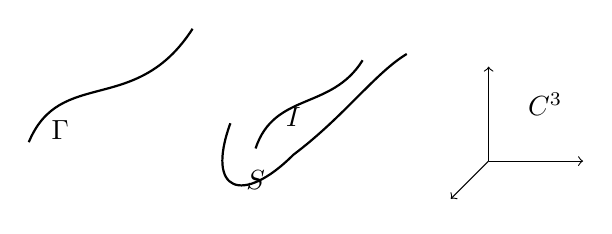
\begin{tikzpicture}[scale=.8]
\draw[thick] (0,0) .. controls (.5,1.2) and (1.7,.4) .. (2.6,1.8);
\node at (.5,.2) {$\Gamma$};
\draw[thick] (3.2,.3) .. controls (2.8,-.8) and (3.4,-1) .. (4.2,-.2) .. controls (5,.4) and (5.5,1.1) .. (6,1.4);
\draw[thick] (3.6,-.1) .. controls (3.9,.8) and (4.8,.5) .. (5.3,1.3);
\node at (3.6,-.6) {$S$};\node at (4.2,.4) {$I$};
\draw[->] (7.3,-.3)--(8.8,-.3);
\draw[->] (7.3,-.3)--(7.3,1.2);
\draw[->] (7.3,-.3)--(6.7,-.9);
\node at (8.2,.6) {$\mathbb C^3$};
\end{tikzpicture}
\end{center}

撇开 $\mathbb C$，若 $k$ 为任意交换域，$\Spec k$ 只含一个点，这一点是整个 $\Spec k$ 的一般点。因此，我们再次看到，不可能从 $\Spec k$ 恢复 $k$！

\textbf{$2^\circ$ $\Spec\mathbb Z$ 与局部环的谱。}

$\mathbb Z$ 是 $\G$ 的始对象，所以来看看 $\Spec\mathbb Z$！有 $(0)\in\Spec\mathbb Z$，因为零理想为素理想当且仅当 $\mathbb Z$ 是整环。$(0)$ 是 $\Spec\mathbb Z$ 的一般点。其他点都形如 $(p)$，其中 $p$ 是素数，$p=2,3,5,7,11,\ldots$。\footnote{译注：原文素数表中的 $11$ 误印为 $10$。}每个这样的 $(p)$ 都是极大理想，即 $\Max\mathbb Z=\{(p)\mid p\text{ 为素数}\}$。因此，每个 $(p)$ 都是闭点。

最后一个例子是极大理想为 $\mathfrak m$ 的局部环 $A$ 的谱 $\Spec A$。尽管这些环一般不具有 $\mathbb C[\xi_1,\xi_2,\ldots,\xi_n]$ 的形式，古典代数几何中也已经考虑过它们。因此，

% PDF 116
\sourcepage{112}{116}
除平凡情形外，$\Spec A$ 与 $\Spec\mathbb C[\xi_1,\ldots,\xi_n]$ 非常不同。事实上，$\Spec A$ 只含唯一闭点 $\mathfrak m$。其他每个点 $\mathfrak p\in\Spec A$ 都是 $\mathfrak m$ 的一般化，即 $\mathfrak m\in\overline{\{\mathfrak p\}}$。在古典代数几何中，若 $Y$ 是复不可约代数簇 $X$ 的一个不可约子簇，则 $A(X)$ 关于素理想 $\mathfrak p_Y$ 的局部化（见第8节）为局部环 $A_Y$；$\Spec A_Y$ 的点与满足 $Y\subset Z\subset X$ 的全部不可约子簇 $Z$ 一一对应。

\textbf{一般性概念的历史演变。}

在意大利学派时期，若不可约的仿射或射影代数簇 $X$ 上的性质 $P$ 只在某个真子簇 $Y\subsetneq X$ 上不成立，就说 $P$“对一般点成立”。用今天的语言，这等价于说 $P$ 在 $X$ 的某个扎里斯基闭集上不成立，或者说 $P$ 在某个扎里斯基开集上成立。例如，“平面 $X$ 中一对一般的有序点恰在唯一一条直线上”，是说该性质仅在对角线 $\{(x,x)\mid x\in X\}$ 上不成立；而对角线是 $X\times X$ 的扎里斯基闭子集。这种惯用说法，类似于实分析中性质“几乎处处成立”，即除去一个零测集后成立。

范德瓦尔登为任意 $X_k\subset k^n$（$k$ 为基域）引入他的“代数点” $(\xi_1,\xi_2,\ldots,\xi_n)$，把它看作表示 $X$ 的 $k$-代数的一组生成元；其特征性质是：取 $k$ 的任意扩域 $\Omega$，其中的点 $\xi$ 为 $X$ 的一般点，当且仅当：1）对每个在 $X$ 上恒为零的 $f$，都有 $f(\xi)=0$；2）对 $X$ 的任意其他点 $x$，都有 $f(\xi)=0\Rightarrow f(x)=0$。这种代数点旨在将意大利学派先前的说法“代数化”，因为那时“一般”点并没有真正的定义。不过显然，它使用了坐标，而且并不唯一。

格罗滕迪克的一般点概念，则给 $\Spec A$ 的每个不可约闭子集配以唯一的一般点；这个点是“内在的”，无须仿射嵌入。正文中由 $Y=\overline{\{x\}}$ 定义的 $Y$ 的一般点 $x$，因而是纯拓扑概念。由扎里斯基拓扑的定义，对任意特化 $y\in\overline{\{x\}}$，仍有 $f(x)=0\Rightarrow f(y)=0$，与范德瓦尔登的情形一样。

\PartTitle{第二部分}{仿射概形上的层}
\Section{6}{引言}
假定读者已知拓扑空间上阿贝尔群层、环层等的主要性质（见原书第6页“预备知识”）。我认为，标准教材 Godement 以及 EGA 的补充材料，对初学者而言都过于庞大；它们是参考书。篇幅适中、证明完整的简明入门，首推塞尔的 FAC 论文（Hirzebruch 的概述，或 Gunning--Rossi 中较详细的介绍，也还算“简短”）。附录（第14节）给出集合层的简短介绍。
% PDF 117
\sourcepage{113}{117}
\begin{quote}
第三章第二部分的主要结果是：利用局部化 $A_{\mathfrak p}$（$\mathfrak p\in\Spec A$）在 $\Spec A$ 上定义结构层，使之成为局部赋环空间 $(\Spec A,\widetilde A)$（见第一章第0节，原书第5页）；$A$ 则成为 $\widetilde A$ 的整体截面环。这样，就从 $A$ 所对应的仿射概形恢复了 $A$。

仿射概形范畴 $\Aff$ 是局部赋环空间范畴的全子范畴。$\Aff$ 同构于含幺交换环范畴 $\G$ 的反范畴 $\G^{\op}$。
\end{quote}

若要从 $X$ 恢复 $A$，$X$ 上的拓扑结构（亦即把它视为拓扑空间）只占所需结构的一小部分。事实上，$X$ 还是赋环空间。\footnote{定义见绪论原书第0--4页脚注(8)；另见 EGA，Springer 版，第0章第4节“Espaces annel\'es”，第87页。态射将在第7节定义。}我们将构造协变函子 $\Aff\to\mathsf{Lrs}$，从仿射代数空间范畴到局部赋环空间范畴。\footnote{$\mathsf{Lrs}$ 的对象是赋环空间 $(X,\mathcal O_X)$，其结构层 $\mathcal O_X$ 的各茎为局部环；也就是说，对每个 $x\in X$，茎 $\mathcal O_{X,x}$ 都是局部环。$\mathsf{Lrs}$ 中的态射将在第7节相应定义。}等价地，这是从含幺交换环范畴 $\G$ 到 $\mathsf{Lrs}$ 的反变函子。

现在来定义早先允诺的额外结构：在 $A$ 的谱上定义一个环层 $\mathcal O_X=\widetilde A$，称为 $X$ 的\textbf{结构层}。

［具备 FAC 中层论基本知识的读者，可以这样理解这一构造。$\widetilde A$ 在点 $\mathfrak p\in\Spec A$ 的茎 $\widetilde A_{\mathfrak p}$ 为归纳极限
\begin{equation}\tag{6.1}
\widetilde A_{\mathfrak p}=\varinjlim_{\substack{U\in\Ob\mathcal B\\\mathfrak p\in U}}A_U,
\end{equation}
其中 $A_U$ 是 $A$ 的局部化环，\footnote{显然，读者需要了解局部化理论。这已是许多研究生代数课程的标准内容；详见 Lang、Atiyah--Macdonald 或 Bourbaki 的交换代数。格罗滕迪克在需要时回顾了主要定义，我把它们集中放在第8节。}$U$ 遍历 $\Spec A$ 的基开集范畴 $\mathcal B$（见本章第3节）。\footnote{另见第3节。译注：(6.1) 原印的极限下标只列 $U\in\Ob\mathcal B$；取茎时须限于含 $\mathfrak p$ 的基开邻域，译文将这一条件显式补出。}$A_U$ 由典范同态 $S_U:A\to A_U$ 及如下泛性质刻画：若 $U=X_f$，则 $S_U(f)$ 在 $A_U$ 中可逆。原文把它称为 $A$ 的“最大同态像”。］

% PDF 118
\sourcepage{114}{118}
$\widetilde A$ 在基开集 $U$ 上的连续截面环同构于 $A_U$。若 $U=X_f$，则 $A_U\simeq A_f$；换言之，对 $U$ 的任意生成元 $f$，$A_U$ 中任一分式 $a/s$ 都可以写成 $a/f^n$。\footnote{回顾 $X_{fg}=X_f\cap X_g$，即 $\mathcal B$ 对有限交封闭。为定义 (6.1) 的“芽”，只考虑 $\mathcal B$ 即已足够，无须考虑整个 $\operatorname{Op}(X)$，因为 $\mathcal B$ 是余终的。$A_f=S_f^{-1}A$ 表示以乘法集 $S_f=\{f^n\mid n\geq0\}$ 中元素为分母的分式 $a/f^n$ 所成的环。}特别地，$f=1$ 时，$X_1=X$，从而 $A_1=A$；于是把 $A$ 恢复为结构层 $\widetilde A$ 在 $X$ 上的整体连续截面环。

\textbf{注。}FAC 的方法一开始就使用茎，可以独立于预层定义层。这也解释了各种语言中用于“纤维” $p^{-1}(x)$ 的农业用语（faisceaux、Garben 等）。格罗滕迪克则把层定义为满足某些正合性条件的特殊预层。理由是技术性的：他的“景”（即格罗滕迪克拓扑）中，对象 $X$ 未必有点，因而也未必有“纤维”或茎 $p^{-1}(x)$。第7节将简要说明两种观点的等价性。第8节回顾分式环的基本事实，以便详细理解 $\widetilde A$ 以及由 $A$-模 $M$ 构造相应 $\widetilde A$-模层的方法。
\begin{center}
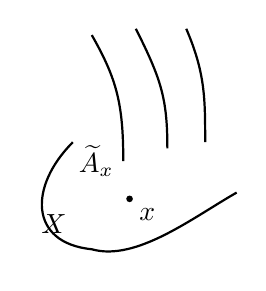
\begin{tikzpicture}[scale=.8]
\draw[thick] (0,1) .. controls (-.7,.3) and (-.7,-.6) .. (.3,-.7) .. controls (1,-.9) and (1.9,-.2) .. (2.6,.2);
\node at (-.3,-.3) {$X$};\fill (.9,.1) circle (1.5pt);\node[below right] at (.9,.1) {$x$};
\draw[thick] (.3,2.7) .. controls (.7,2) and (.8,1.6) .. (.8,.7);
\draw[thick] (1,2.8) .. controls (1.4,2) and (1.5,1.7) .. (1.5,.9);
\draw[thick] (1.8,2.8) .. controls (2.1,2.1) and (2.1,1.7) .. (2.1,1);
\node[left] at (.8,.7) {$\widetilde A_x$};
\end{tikzpicture}
\end{center}

设 $M$ 是任意 $A$-模。可以构造 $\widetilde A$-模层 $\widetilde M$，使它在每个 $\mathfrak p\in\Spec A$ 处的茎为局部化模 $M_{\mathfrak p}$。实际上，$\widetilde A$ 与 $\widetilde M$ 的构造可以同时进行，因为把 $A$ 看作自身上的 $A$-模时，环的局部化理论就是模的局部化理论的特例。反过来，若 $\mathcal M$ 是任意 $\widetilde A$-模层，即对每个 $x\in\Spec A$，$\mathcal M_x$ 都是 $\widetilde A_x$-模，自然要问：$\mathcal M$ 是否来自某个 $A$-模？这当且仅当 $\mathcal M$ 是拟凝聚 $\widetilde A$-模层。

依据课堂录音整理的 $\widetilde A$ 的实际构造见第9节。第7、8节提供预备材料；熟悉这些知识的读者可以从第9节读起。

［这样，终于可以定义仿射概形范畴 $\G'$。事实上，它同构于代数空间范畴 $\Aff$（见第一章），亦即 $\G$ 上可表函子的范畴；或者等价地，可以把仿射概形与 $\G$ 的反范畴的对象等同起来。

具体地，给每个含幺交换环 $A\in\Ob\G$ 配以仿射概形 $(\Spec A,\widetilde A)$，即这样一个局部赋环空间：底拓扑空间是赋有谱拓扑的 $\Spec A=\{\mathfrak p\mid\mathfrak p\text{ 是 $A$ 的素理想}\}$，结构层 $\widetilde A$ 则是刚才提到的各茎为局部环 $A_{\mathfrak p}$（$\mathfrak p\in\Spec A$）的层。我们将

% PDF 119
\sourcepage{115}{119}
看到，$(\Spec A,\widetilde A)$ 能恢复 $A$。\footnote{例如，最简单的情形是 $A=k$ 为域，此时 $(\Spec k,\widetilde k)=(\{(0)\},k)$。}此外，若 $f:A\to B$ 是 $\G$ 中任意态射，则有一个方向相反、良定义的局部赋环空间态射
\[
(\Spec B,\widetilde B)\longrightarrow(\Spec A,\widetilde A).
\]
它包含底拓扑空间之间的连续映射 $\Spec B\to\Spec A$，以及一个再次反向的层同态。

应当强调，$A$ 可以约化，也可以不约化。］

\Section{7}{FAC 与格罗滕迪克观点下的层；赋环空间}
我认为 FAC 已经相当为人熟知，它可以作为从古典代数几何过渡到格罗滕迪克代数几何的准备。FAC 不先引入预层，而是直接定义层；下面说明两种方法等价。

按照 FAC，拓扑空间 $X$ 上的阿贝尔群层\footnote{环层、局部环层、集合层等可以类似定义。}，是另一个拓扑空间 $S$ 到 $X$ 的平展覆盖 $p:S\to X$，\footnote{在这里，“平展覆盖”只是说投影 $p:S\to X$ 为局部同胚：每个 $s\in S$ 都有开邻域 $U\ni s$，使 $p|_U:U\to p(U)$ 为同胚。详见附录。}使得对每个 $x\in X$，茎 $S_x=p^{-1}(x)$ 都是阿贝尔群，而且由
\begin{equation}\tag{7.1}
(a,b)\longmapsto a-b
\end{equation}
定义的映射 $S\times_XS\to S$ 连续。\footnote{按 FAC 的层定义，$S\times S$ 赋予乘积拓扑，$S\times_XS$ 赋予诱导拓扑。另参见第二章第3节。译注：正文原印把差映射的目标误写为 $X$，应为 $S$。}

FAC 中有两种方式比较层与预层。若 $S$ 是层，则给每个开集 $U\subset X$ 配以连续截面阿贝尔群的对应 $U\mapsto\Gamma(S|_U)$，\footnote{层 $S$ 在开集 $U\subset X$ 上的连续局部截面，是满足 $p\circ s=1_U$ 的连续映射 $s:U\to S$。}构成一个预层（见第3节），称为 $S$ 所定义的\textbf{典范预层}，或\textbf{连续局部截面预层}。另一方面，若 $P$ 是任意阿贝尔群预层，可以对开集 $U$ 上的元素 $f\in P(U)$ 定义它在 $x\in X$ 处的芽，其中

% PDF 120
\sourcepage{116}{120}
$x\in U$。其定义使用熟知的等价关系，也可写成归纳极限
\[
P_x=\varinjlim_{U\ni x}P(U).
\]
再以不交并 $S_P=\coprod_{x\in X}P_x$ 为底集，赋予自然拓扑，构造 $X$ 上预层 $P$ 的极限层，使 $S_P$ 成为 $X$ 的平展覆盖，且代数运算连续。

层范畴 $\operatorname{Top}(X)$ 与预层范畴 $\operatorname{Presh}(X)$ 之间的这两个函子并不互逆。确切地说，预层 $P$ 的极限层 $S_P$ 的连续局部截面预层 $\mathcal P$，一般不能与 $P$ 典范等同；只有典范映射 $P\to\mathcal P$。于是自然要刻画那些能与 $S_P$ 的典范预层等同的预层 $P$。FAC 已经提出并解决了这一问题，答案可以用一个正合性条件刻画：

\textbf{预层 $F$ 是典范预层，当且仅当对每个开覆盖 $U=\bigcup_{i\in I}U_i$，下列图式正合：}
\begin{equation}\tag{7.1}
F(U)\longrightarrow\prod_{i\in I}F(U_i)
\rightrightarrows\prod_{i,j\in I}F(U_i\cap U_j).
\end{equation}
\footnote{译注：本式与前页的差映射在原文中重复使用编号 (7.1)，这里保留原编号。}
建议把这一正合性条件涉及的两项验证用文字表述出来，看看它们正好给出典范层的两个熟知条件：
\begin{enumerate}[label=\alph*)]
\item $F$ 是\textbf{分离的}：$F(U)$ 中的截面由它在覆盖各部分上的限制唯一确定。
\item $F$ 是“\textbf{局部的}”：给定各 $U_i$ 上的截面，只要满足“相容条件”，就存在一个截面（由 a) 可知唯一），其在每个 $U_i$ 上的限制恰为给定截面。
\end{enumerate}

% PDF 121
\sourcepage{117}{121}
$X$ 上的层范畴 $\operatorname{Top}(X)$ 和预层范畴 $\operatorname{Presh}(X)$ 之间的两个函子\footnote{$\operatorname{Presh}(X)$ 中的态射是自然变换。按 FAC 定义的两个层 $p:S\to X$、$q:T\to X$ 之间的态射，是使三角形 $S,T,X$ 交换，并对每个 $x\in X$ 诱导纤维同态 $S_x\to T_x$ 的连续映射 $S\to T$。}
\[
\begin{tikzcd}[column sep=large,ampersand replacement=\&]
\operatorname{Top}(X)\arrow[r,bend left=15,"i"]\&
\operatorname{Presh}(X)\arrow[l,bend left=15,"\gamma"]
\end{tikzcd}
\qquad(i\text{ 为包含函子，$\gamma(P)$ 为典范层})
\]
互为伴随（见第二章）。也就是说，若 $S$ 是层、$P$ 是预层，原文给出典范等同
\begin{equation}\tag{7.2}
\Hom_{\operatorname{Top}(X)}(S,\gamma(P))
\simeq\Hom_{\operatorname{Presh}(X)}(i(S),P).
\end{equation}
\footnote{译注：原文把伴随方向颠倒了。层化 $\gamma$ 是包含函子 $i$ 的左伴随，正确的式子为 $\Hom_{\operatorname{Top}(X)}(\gamma(P),S)\simeq\Hom_{\operatorname{Presh}(X)}(P,i(S))$。}

在本课程以及大多数著作中，格罗滕迪克都采用正合性条件来定义层，因为它更具有范畴性：可以把 $\operatorname{Op}(X)$ 换成任意具有纤维积的范畴。概括地说，$X$ 上的层就是满足上述正合性条件的预层。

这种方法中，“茎”不显式出现；但对任意“景”（亦即格罗滕迪克拓扑）而言，这恰好方便，因为在那里茎并不居于首要地位。

格罗滕迪克代数几何的主要研究对象——概形，是赋环空间的特殊情形。赋环空间即配有环结构层 $\mathcal O_X$ 的拓扑空间 $X$，记为二元组 $(X,\mathcal O_X)$。读者至少在直观上已经熟悉的最简单例子，是各类流形\footnote{并不假定读者具有流形的专门知识。只须回忆“大学一年级微积分”中的例子，把曲线或曲面换成 $n$ 维流形即可。}（为明确起见，以下考虑拓扑流形或 $C^\infty$ 可微流形）。例如，考虑曲面 $X$。$X$ 上的局部实值函数构成预层
\[
U\longmapsto\Gamma(U,\mathcal O_X),
\]
其中 $U$ 在 $X$ 中开，而 $\Gamma(U,\mathcal O_X)$ 是函数 $U\to\mathbb R$ 所成的环。

% PDF 122
\sourcepage{118}{122}
两个曲面之间的映射 $F:(X,\mathcal O_X)\to(Y,\mathcal O_Y)$，意指将局部函数变为局部函数的连续映射 $F:X\to Y$。由于函数按反变方式作用，唯一合理的做法是把局部函数 $\varphi:U\to\mathbb R$（$U$ 为 $Y$ 的开集）拉回为局部函数
\[
\varphi\circ F:F^{-1}(U)\longrightarrow\mathbb R.
\]
$F$ 连续，所以 $F^{-1}(U)$ 在 $X$ 中开。更精确地，有一个环同态
\[
\Gamma(U,\mathcal O_Y)\longrightarrow\Gamma(F^{-1}(U),\mathcal O_X).
\]
\begin{center}
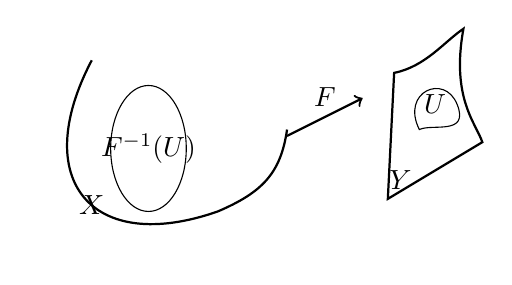
\begin{tikzpicture}[scale=.8]
\draw[thick] (0,1.7) .. controls (-1,-.2) and (0,-1.4) .. (2,-.7) .. controls (2.7,-.4) and (3,-.1) .. (3.1,.6);
\draw (.9,.3) ellipse (.6 and 1);
\node at (.9,.3) {$F^{-1}(U)$};\node at (0,-.6) {$X$};
\draw[->,thick] (3.1,.5)--(4.3,1.1) node[midway,above] {$F$};
\draw[thick] (4.7,-.5)--(4.8,1.5) .. controls (5.3,1.6) and (5.6,2) .. (5.9,2.2) .. controls (5.7,1.1) and (6.1,.7) .. (6.2,.4)--cycle;
\draw (5.2,.6) .. controls (4.9,1.2) and (5.6,1.5) .. (5.8,1) .. controls (6,.5) and (5.4,.7) .. cycle;
\node at (5.45,1) {$U$};\node at (4.9,-.2) {$Y$};
\end{tikzpicture}
\end{center}

而且，这一运算与芽的构造相容；芽是 $\varinjlim_{U\ni x}\Gamma(U)$ 的元素。下面明确写出这一构造。

设 $f_U:U\to\mathbb R$、$f_V:V\to\mathbb R$ 是定义在 $x$ 的两个开邻域上的局部函数。\footnote{视具体情形，函数取连续的（$C^0$）或 $C^\infty$ 的。$C^0$ 情形自动成立，$C^\infty$ 情形则带来较强限制：不能要求拉回任意函数 $\varphi$，这里只拉回 $C^\infty$ 函数。}若存在第三个开邻域 $W$，$x\in W\subset U\cap V$，使 $f_U|_W=f_V|_W$，则记 $f_U\sim f_V$。容易验证，$\sim$ 的确是所有定义在 $x$ 的开邻域上的局部函数所成集合上的等价关系，并且与环运算相容。
\begin{center}
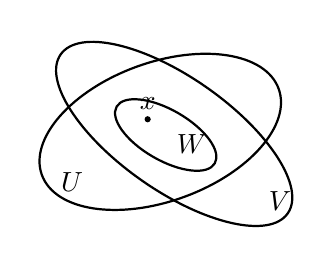
\begin{tikzpicture}[scale=.8]
\draw[thick,rotate=20] (0,0) ellipse (2 and 1.1);
\draw[thick,rotate=-35] (.2,.1) ellipse (2.2 and .9);
\draw[thick,rotate=-30] (.1,0) ellipse (.9 and .4);
\fill (-.2,.2) circle (1.4pt);\node[above] at (-.2,.2) {$x$};
\node at (.5,-.2) {$W$};\node at (-1.4,-.8) {$U$};\node at (1.9,-1.1) {$V$};
\end{tikzpicture}
\end{center}
由 $f_U$ 所定义的等价类称为 $f_U$ 在 $x$ 处的\textbf{芽}。$x$ 处的芽用大写花体字母 $\mathcal F,\mathcal G,\mathcal H,\ldots$ 表示，并在左下方标出 $x$，即 ${}_x\mathcal F,{}_x\mathcal G,{}_x\mathcal H,\ldots$。不要把芽与实数 ${}_x\mathcal F(x)$（芽在 $x$ 处的值）混淆；这个值有意义，因为
\[
f_U\sim f_V\Longrightarrow f_U(x)=f_V(x).
\]
\footnote{但若 $y\ne x$，就不能定义 ${}_x\mathcal F(y)$。}
